%-------------------------------------------------------
\section{Pre-crisis Vulnerabilities}
%-------------------------------------------------------

\begin{frame}

\begin{center}
{\LARGE Pre-crisis Vulnerabilities}
\end{center}

\end{frame}

%-------------------------------------------------------

%-------------------------------------------------------

\begin{frame}{Pre-crisis vulnerabilities}

\begin{figure}
\begin{center}

\resizebox{0.65\textwidth}{!}{%
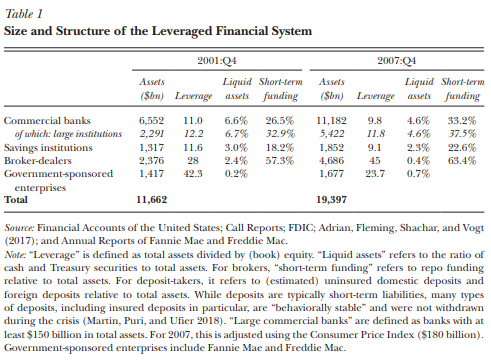
\includegraphics{Figures/aikman_et_al_banks_bs_pre_crisis.png}
}

\caption{\label{fig:L4_aikman_et_al_banks_bs_pre_crisis} Buildup of vulnerabilities from $2001$ to $2007$ - solvency, liquidity and funding. Source: \href{https://pubs.aeaweb.org/doi/pdfplus/10.1257/jep.33.1.107}{Aikman \emph{et al} (2019)}}

\end{center}
\end{figure}

%The most extreme vulnerabilities developed for the parts of the financial
%system that did not take traditional deposits. Consider, for instance, the changes
%for broker-dealers, a category that includes specialised investment banks and the
%investment banking subsidiaries of larger banking groups. The assets of these entities increased from 28 to 45 times their equity between 2001 and 2007, meaning that
%a roughly 2 percent decline in the value of broker-dealers’ assets would have been
%sufficient to wipe out all of their equity. In addition, these firms were traditionally
%highly reliant on short-term wholesale funding (Rosengren 2014), and became even
%more so during this period.
%Much of this short-term funding took the form of repurchase agreements, or
%“repos.” Repos are a form of borrowing in which the broker-dealer sells securities
%that it holds, receives the value of those securities in cash, and a few days later repurchases the securities at a predetermined price that includes an additional interest
%payment. The repo liabilities of broker-dealers increased from $1.4 trillion in 2001
%to $3.0 trillion in 2007.1
% Moreover, an increasing fraction of repos were backed by
%low-quality securities. 

\end{frame}

%-------------------------------------------------------

%-------------------------------------------------------

\begin{frame}{Off balance sheet exposures}

\begin{figure}
\begin{center}

\resizebox{0.70\textwidth}{!}{%
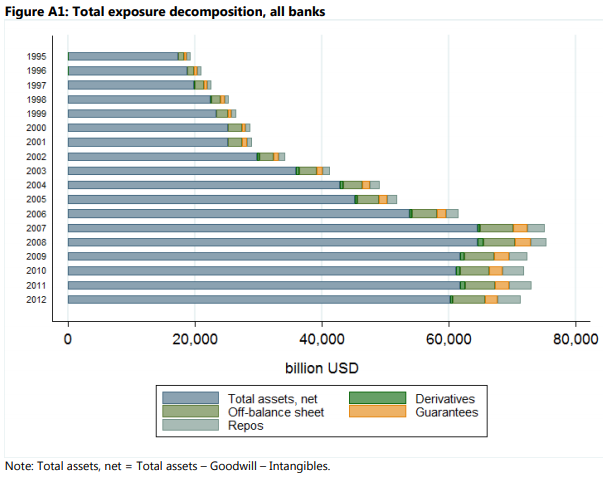
\includegraphics{Figures/total_exposure_incl_derivs_off_bs.png}
}

\caption{\label{fig:L4_total_exposure_incl_derivs_off_bs} Adjusting total exposure for derivatives and off-balance-sheet positions. Source: \href{https://www.bis.org/publ/work471.pdf}{Brei and Gambacorta (2014)}}

\end{center}
\end{figure}

\end{frame}

%-------------------------------------------------------

%-------------------------------------------------------

\begin{frame}{Risk weight `optimization' (regulatory arbitrage)}

\begin{figure}
\begin{center}

\resizebox{0.70\textwidth}{!}{%
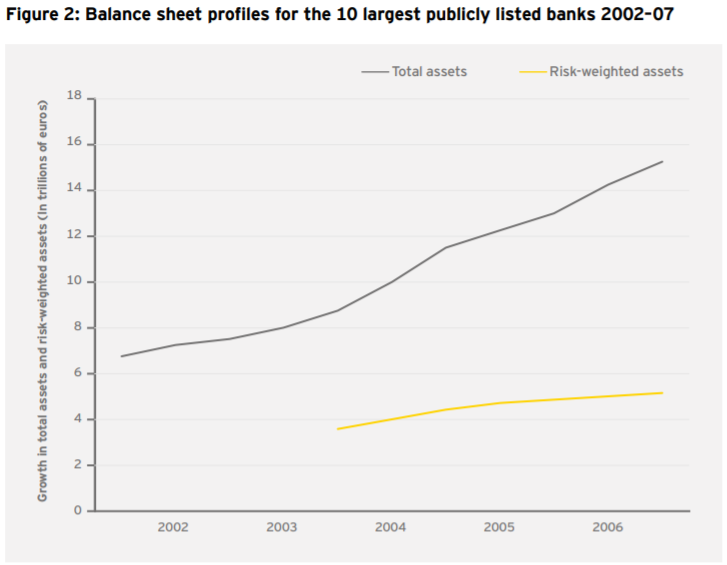
\includegraphics{Figures/ey_ta_rwa_note.png}
}

\caption{\label{fig:L4_ey_ta_rwa_note} Approximate constancy of capital ratios with respect to risk weighted assets vs. buildup of leverage. Source: EY, Avgouleas and Cullen (2015); IMF}

\end{center}
\end{figure}

%While asset levels increased markedly in the years leading up to the GFC, reported leverage
%levels at large commercial banks were remarkably constant. This would normally suggest
%that while banks expanded asset levels aggressively they maintained capital levels and
%preserved stable leverage ratios [Kalemli-Ozcan et al. (2012)]. However, official data
%does not provide the full picture. Leverage increases were caused by poorly calibrated
%internal financial models [Simkovic (2009)], the poor performance of credit rating agencies
%[Johnston (2011)], and fraud [Valukas (2010)].
%Moreover, there is strong evidence that reported leverage levels at both commercial and
%investment banks were manipulated, or were inaccurate, due to exploitation of prevalent
%rules on bank capital by bank management. For example, banks switched away from loans
%into structured financial products, which benefitted from higher capital relief. The increased
%role of complex securitized credit and marketable securities provided additional avenues
%to augment bank capital structures [Stein (2010)]. Under the Basel Accords, the lower risk
%weights that securitized products attracted meant that banks did not have to hold the same
%levels of capital against those assets, as it would be the case if the underlying products were
%not securitized. Basel II, in particular, made few significant changes to regulatory capital
%requirements in relation to conduits, leading to a reduction in overall capital requirements.
%Much risk-weighted optimization (RWO) was achieved through employment of securitization
%models, as it was assumed that by diversifying and spreading risk throughout the financial
%system through securitization, the financial system would be more stable and more resilient
%to shocks [Blair (2013)]. These conduits raised funds by selling short-term asset-backed
%commercial paper, with the assets concerned usually comprising mortgage pools and
%secured loans. Because these conduits funded themselves with short-term debt, any loss of
%confidence or liquidity pressures due to a reduction in buyers of commercial paper would
%quickly destroy their viability, indirectly exposing the sponsor bank to funding liquidity risk.
%The dual advent of risk-weighted capital requirements and financial innovation for funding
%has hereto enabled banks to engage in RWO for the best part of the past two decades.
%Indeed, research confirms that RWO has not abated since the GFC [Blundell-Wignall and
%Atkinson (2012)]. This has resulted in several large European banks operating with relatively
%low levels of common equity, despite being “well-capitalized” in terms of tier-1 risk-based
%capital (Figure 3).

\end{frame}

%-------------------------------------------------------

%-------------------------------------------------------

\begin{frame}{Enormous expansion of leverage}

Banks (and other financial intermediaries) were highly levered
	\begin{itemize}
	\item	Especially if one looks at raw (not risk-weighted) assets
	\end{itemize}
\vspace{2mm}
Plentiful supply of funds
	\begin{itemize}
	\item	Partly a search for yield
	\item	Developing countries - esp. oil producers - looking to invest using their `savings glut'
	\end{itemize}
\vspace{2mm}
Misspricing and unawareness of risks of innovative, opaque and poorly understood asset classes which often collateralized debt
	\begin{itemize}
	\item	Regulators, risk weights
	\item	Ratings agencies
	\item	Market participants
	\end{itemize}
\vspace{2mm}
Also reflected highly profitable (for a time) `originate and distribute' model\ldots
	
\end{frame}

%-------------------------------------------------------

%-------------------------------------------------------

\begin{frame}{Originate and distribute}

Traditionally banks originated loans and then held them on their balance sheet
\begin{itemize}
\item	Incentive to keep monitoring them and make good loans to begin with
\end{itemize}
\vspace{2mm}
Arguably the `market' can improve on this
\begin{itemize}
\item	Banks may not be the natural holders of the various types of risks involved - even if they are good at originating loans (vetting borrowers etc.)
\end{itemize}
\vspace{2mm}
Securitization (supposedly) allowed banks to `distribute' the loans
	\begin{itemize}
	\item	Shift a pool of loans to special purpose vehicles (SPVs)
	\item 	SPVs issue asset backed commercial paper (or MBS if they were pools of mortgages)
	\item	This CP allows the loans to be funded `off balance sheet' of the bank (with perhaps an explicit or implicit back-up line of credit)
	\end{itemize}

\end{frame}

%-------------------------------------------------------

%-------------------------------------------------------

\begin{frame}{Originate and distribute}

Why might OaD promote lending? Optimistic answer\ldots
	\begin{itemize}
	\item	Improves liquidity (lowers borrowing rates)
		\begin{itemize}
		\item	Might allow banks to de-risk or raise funds more quickly under stress
		\item	See Loutskina (2011) and Bidder \emph{et al} (2019)
		\end{itemize}
	\vspace{2mm}
	\item	Reduces risk through diversification and a broader investor base
		\begin{itemize}
		\item	Tranching of asset pools allowed creation of derivative assets with different risk classes
		\item	Some investors (e.g. money market funds) can only invest in AAA
		\item	AAA can be synthesized by `last loss' or `super senior' tranche of CDOs
		\item	Interesting literature on the shortage of public provision of `riskless assets' (see Krishnamurthy and Caballero's work) inducing private sector to fill the void
		\end{itemize}
	\end{itemize}
\vspace{2mm}
\textbf{But banks were buying a lot of the derivatives - so risk was staying within the system!}
\end{frame}


%-------------------------------------------------------

%-------------------------------------------------------

\begin{frame}{Originate and distribute}

Why might OaD promote lending? More cynical (realistic) answer\ldots
	\begin{itemize}
	\item	Preferential regulatory treatment of off-balance sheet item
		\begin{itemize}
		\item	Less capital required despite same risk (possibly endogenously worse)
		\item	Capital held against loans $>$ capital held against backup lines of credit
		\end{itemize}
	\vspace{0.5mm}
	\item	Private securitization (esp. of subprime mortgages and ABCP) helped artificially stimulate credit  - \href{https://academic.oup.com/qje/article-abstract/125/1/307/1880343?redirectedFrom=fulltext}{Keys \emph{et al} (2010)}.
		\begin{itemize}
		\item	Eventually seemed to induce declines in lending standards
		\item	Low-documentation, NINJA and ARMs became prevalent
		\item	Senior Loan Office Surveys also indicated excessive loosening
		\item	Homeowners encouraged to extract equity (aggregate LTV $\approx$ flat despite price rises)	
		\end{itemize}
	\end{itemize}

\vspace{2mm}
Research by \href{https://academic.oup.com/qje/article-abstract/128/4/1687/1849337}{Mian and Sufi (2013)} $\Rightarrow$ debt was an important transmission mechanism to the broader economy
		\begin{itemize}
		\item	Fine until \textbf{aggregate} U.S. house prices slowed/turned
		\item	Overleveraged households (or states where they were prevalent) suffered the most when the cycle turned
		\end{itemize}
	
\end{frame}

%-------------------------------------------------------

%-------------------------------------------------------

\begin{frame}{Mortgage debt and house price growth (and collapse)}

\begin{figure}
\begin{center}

\resizebox{0.60\textwidth}{!}{%
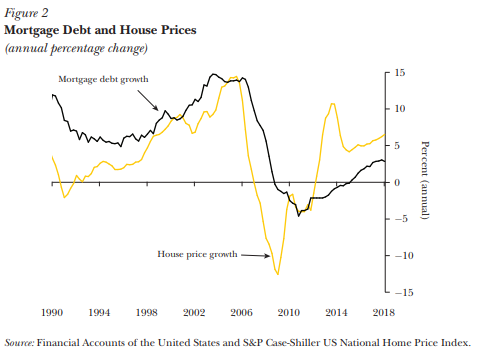
\includegraphics{Figures/aikman_et_al_house_prices_mortage.png}
}

\caption{\label{fig:L4_aikman_et_al_house_prices_mortage} Rapid run-up (and then crash) in mortgage debt growth and U.S. house prices. Source: \href{https://pubs.aeaweb.org/doi/pdfplus/10.1257/jep.33.1.107}{Aikman \emph{et al} (2019)}}

\end{center}
\end{figure}

%Mortgage debt doubled in the six years before the
%crisis, and by 2007 reached 72 percent of GDP. Two aspects of this debt build-up are
%noteworthy and will inform our later macroprudential analysis.
%First, the increase in mortgage debt was accompanied by a house price boom,
%shown in Figure 2. House prices rose by two-thirds in the five years to their peak in
%early 2006 (according to the S&P Case-Shiller US National Home Price Index), and
%ongoing rapid house price appreciation was embedded in expectations (Gennaioli
%and Shleifer 2018). The aggregate loan-to-value ratio on the stock of US housing
%remained broadly flat during this period, meaning that for each 1 percent increase
%in house values, homeowners also increased their mortgage debt by around
%1 percent. In part, this reflected new homeowners taking out larger mortgages in
%order to purchase more expensive homes. But in addition, existing homeowners
%also extracted housing equity by taking out additional debt. Mian and Sufi (2011)
%estimate that existing homeowners borrowed $0.25 on average for every $1 increase
%in home-equity value during the housing boom, enough to account for over half of
%the increase in debt for homeowners between 2002 and 2006.
%Second, there were clear signs in the years before the financial crisis that lending
%standards were being loosened and borrower quality was deteriorating. The Federal
%Reserve Board’s Senior Loan Officer Opinion Survey on Bank Lending Practices
%reported easing standards between 2004Q1 and 2006Q3. The expansion of credit to
%the most risky borrowers was particularly pronounced. For example, according to the
%Federal Reserve’s Survey of Consumer Finances, the share of the stock of mortgagors
%with debt of over four times their income more than doubled between 2001 and 2007
%from 6 percent to 13 percent. The number of new subprime mortgages nearly doubled
%between 2003 and 2005, 80 percent of which were made with short-term “teaser” interest
%rates (in this journal, Mayer, Pence, and Sherlund 2009). “Near-prime” mortgages also
%increased rapidly. The private-label securitization market, in which these mortgages
%were bundled into tranched financial securities and resold, was an important driver of
%these frothy credit supply conditions (Keys, Mukherjee, Seru, and Vig 2010).

\end{frame}

%-------------------------------------------------------

%-------------------------------------------------------

\begin{frame}{Commercial paper buildup - especially asset-backed}

\begin{figure}
\begin{center}

\resizebox{0.70\textwidth}{!}{%
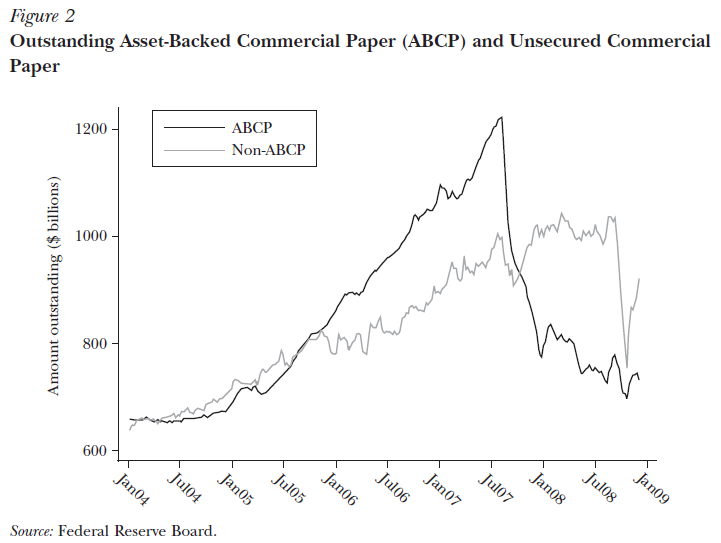
\includegraphics{Figures/ABCP_cliff.png}
}

\caption{Buildup and then collapse in ABCP (eventually followed by non-asset backed paper). Source: \href{https://www.princeton.edu/~markus/research/papers/liquidity_credit_crunch.pdf}{Brunnermeier (2009); Bloomberg}}

\end{center}
\end{figure}

\end{frame}

%-------------------------------------------------------

%-------------------------------------------------------

\begin{frame}{Additional vulnerabilities}

Increased opacity of assets and counterparty interlinkages
	\begin{itemize}
	\item	Companies (e.g. AIG) that weren't on the radar, become enormously interlinked through insuring CDOs etc.
	\item	Fine while agents are looking for `informationally insenstive' assets, but disastrous when people were trying to reasses
	\item	In the absence of liquid markets the assets are very difficult to price / learn about - so arbitrary beliefs can be held\ldots
	\end{itemize}
\vspace{2mm}
Shortened maturity of debt (recall Diamond-Dybvig!)
	\begin{itemize}
	\item	Large banks used short maturity repo to roll massive amounts of debt
	\item	No `deposit insurance' for repo!
	\item	$3$-month repo fairly constant but overnight increased substantially
	\item	Tapping money market funds on basis of (implausible) AAA ratings
	\item	Off-balance sheet lines of credit for SPV were a \textit{time bomb}
	\end{itemize}

\end{frame}

%-------------------------------------------------------

%-------------------------------------------------------

\begin{frame}{Additional vulnerabilities}

Repo (or a `repurchase agreement')
	\begin{itemize}
	\item	A form of collateralized borrowing
	\item	Borrower sells an asset to the lender at a `haircut'
	\item	Promises to buy at back at maturity plus interest
	\item	Simple summaries \href{https://www.investopedia.com/terms/r/repurchaseagreement.asp}{here}, \href{https://en.wikipedia.org/wiki/Repurchase_agreement}{here} and \href{https://www.icmagroup.org/Regulatory-Policy-and-Market-Practice/repo-and-collateral-markets/icma-ercc-publications/frequently-asked-questions-on-repo/3-what-is-the-role-of-repo-in-the-financial-markets/}{here} (see also the Gorton-Metrick `run on repo' paper in the readings - early sections)
	\end{itemize}

\end{frame}

%-------------------------------------------------------

%-------------------------------------------------------

\begin{frame}{Additional vulnerabilities}

\begin{figure}
\begin{center}

\resizebox{0.50\textwidth}{!}{%
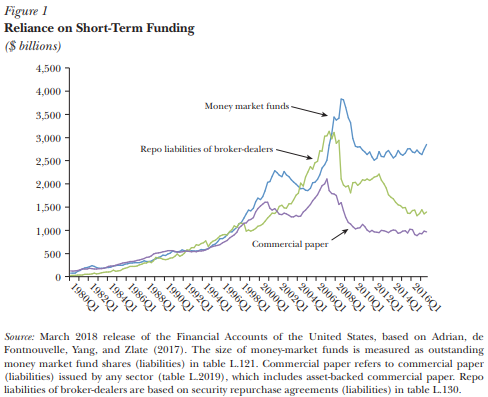
\includegraphics{Figures/aikman_et_al_short_term_funding.png}
}

\caption{\label{fig:L4_aikman_et_al_short_term_funding} Buildup of vulnerabilities from $2001$ to $2007$ - increased use of repo and other short term funding and the absorption of this debt by money market funds. Source: \href{https://pubs.aeaweb.org/doi/pdfplus/10.1257/jep.33.1.107}{Aikman \emph{et al} (2019)}}

\end{center}
\end{figure}

%Figure 1 shows the rise in repo funding, along with commercial paper, another
%form of funding that experienced rapid growth over this period. Traditional commercial paper is short-term debt issued by companies to fund operations. However, by
%the end of 2006, 60 percent of outstanding commercial paper consisted of so-called
%“asset-backed commercial paper” that had been issued to fund the purchase of specific
%securities such as credit card receivables, auto loans, or mortgage-backed securities.
%The growth in repos and commercial paper coincided with an increase in
%the size of money market mutual funds, which purchased much of the repos and
%commercial paper issued. Regulators allowed money market mutual funds to invest
%in assets with a weighted average maturity of up to 90 days, but these funds offered
%investors the ability to withdraw their money at a day’s notice. Moreover, money
%market mutual funds did not have any capital that would shield these short-term
%investors from losses. In a crisis, investors in money market mutual funds who withdrew their funds first were certain to be fully paid, while later claims might not be
%fully paid, providing incentives to “run” on the fund.
%In summary, nonbanks became an increasingly important source of credit for
%the real economy in the years preceding the crisis: between 2001 and 2007, nonbank
%financials accounted for over 70 percent of the total growth in home mortgage
%credit (according to the Financial Accounts of the United States). This growth was
%accompanied by an increased reliance on debt financing of the nonbank system.
%Short-term borrowing became more important, with the belief that it could be rolled over continually

\end{frame}

%-------------------------------------------------------

%-------------------------------------------------------

\begin{frame}{Still dancing\ldots}

\begin{quote}
When the music stops, in terms of liquidity, things will be complicated. But as long as the music is playing, you’ve got to get up and dance. We’re still dancing.
\end{quote}
\begin{center}
- Chuck Prince, Citi CEO, July 10, 2007
\end{center}

\end{frame}